\documentclass[main.tex]{subfiles} % Subfile-Class

%==============================================================================%
%                                   Subfile                                    %
%==============================================================================%

\begin{document}

% Template

\section{Funktionsübersicht}

\subsection{Systemaufbau im Überblick}

Das entwickelte Fahrzeug ist ein autonomer Roboter, der sich selbstständig durch ein 
vordefiniertes Wegenetz zum gewählten Zielpunkt navigiert. Dabei reagiert er 
dynamisch auf Hindernisse, gesperrte Wegpunkte und fehlende Streckenabschnitte. Der 
Systemaufbau folgt einer modularen Struktur und wurde hinsichtlich Gewicht, 
Steuerbarkeit und Wartbarkeit optimiert.

Die \textbf{zentralen Systemkomponenten} sind in Abbildung~\ref{fig:Gesamtuebersicht} 
dargestellt und lassen sich in folgende Hauptgruppen unterteilen:

\begin{itemize}
    \item \textbf{Chassis und Antrieb:} 
    Das Fahrzeug basiert auf einer leichten, vollständig 3D-gedruckten PLA-Konstruktion. 
    Zwei hintere Schrittmotoren treiben speziell entwickelte Felgen mit Vollgummireifen 
    an. Eine freilaufende Laufkugel an der Front sorgt für Stabilität und enge 
    Wendemanöver auf Knotenpunkten. Die kompakte Bauweise mit Distanzbolzen statt 
    Etagenkonstruktion verbessert die Zugänglichkeit aller Komponenten.
    
    \item \textbf{Sensorik:} 
    Zur Umgebungswahrnehmung werden mehrere Sensortechnologien kombiniert: ein 
    UV-basierter Liniensensor zur Spurverfolgung, ein Ultraschallsensor zur 
    Hinderniserkennung, ein LiDAR-Modul zur Detektion gesperrter Wegpunkte (Pylonen) 
    sowie eine Kamera zur Knoten- und Zielerkennung.
    
    \item \textbf{Steuerungseinheit:} 
    Die Logik ist zweistufig aufgebaut: Ein Raspberry Pi 5 übernimmt die Navigation, 
    Bilderkennung und Strategie, während ein Mikrocontroller (Raspberry Pi Pico) unter 
    FreeRTOS für die Echtzeitsteuerung von Antrieb, Greifer und Sensorik verantwortlich 
    ist. Die Kommunikation erfolgt über ein eigenes 64-Bit-UART-Protokoll mit 
    CRC-Fehlerprüfung.
    
    \item \textbf{Greifeinheit:} 
    Die Greifmechanik ist modular konstruiert und besteht aus zwei synchron bewegten 
    Backen mit Anti-Rutsch-Belag. Ein zusätzlicher Servomotor erlaubt die vertikale 
    Positionierung entlang einer Gleitführung. Endschalter sichern die obere und untere 
    Endlage ab. Die gesamte Einheit ist für hohe Wiederholgenauigkeit und minimales 
    Gewicht ausgelegt.
    
    \item \textbf{Energieversorgung:} 
    Ein 4S-LiPo-Akku versorgt das System mit 14.4 V. Die Spannungsaufbereitung erfolgt 
    über ein Power-Board mit 12 V-Ausgang und lokalen Reglern auf jedem PCB. Während 
    der Entwicklung kann über ein externes Netzteil betrieben werden. Ein 
    softwarebasierter Not-Aus unterbricht bei Bedarf alle Bewegungen sofort.
    
    \item \textbf{Benutzerschnittstelle:} 
    Vor Fahrtbeginn kann über einen Wahlschalter das gewünschte Ziel (A, B oder C) 
    eingestellt werden. Nach Zielerreichung gibt ein Piezo-Summer akustisches Feedback. 
    Weitere Schnittstellen wie UART-Debug oder eine einfache GUI stehen für Entwicklungs- 
    und Testzwecke zur Verfügung.
\end{itemize}

Die klare Trennung zwischen Hardware-Ansteuerung und Navigationslogik sowie die modulare 
Konstruktion erlauben einfache Wartung, gezielte Optimierungen und ein robustes Verhalten 
im Wettbewerbsbetrieb.

\begin{figure}[H]
    \centering
    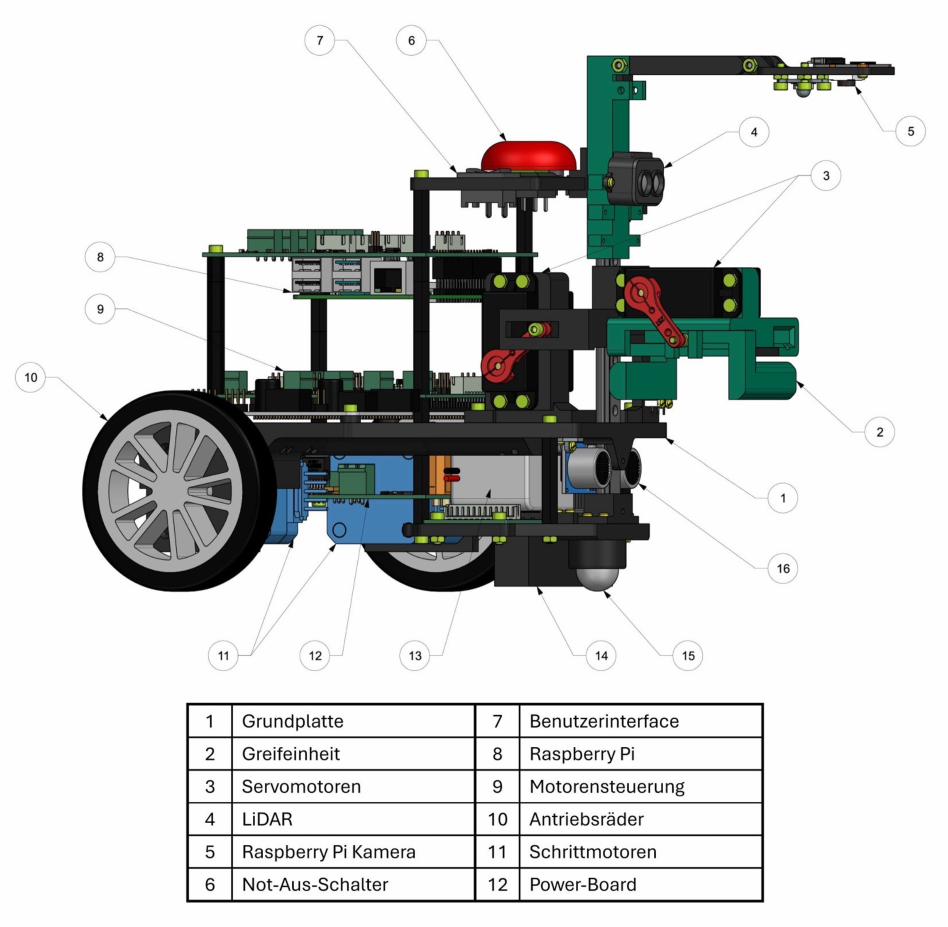
\includegraphics[width = 1.0\linewidth]{./Figures/Gesamtuebersicht-Fahrzeug.pdf}
    \caption{Gesamtübersicht des Fahrzeugs mit Bildlegende}~\label{fig:Gesamtuebersicht}
\end{figure}

\vspace{1em}

\subsection{Navigation und Zielfindung}

Die Navigation basiert auf der kontinuierlichen Verfolgung der Leitlinie mittels einem 
Liniensensor. Knotenpunkte werden automatisch erkannt und das Fahrzeug stoppt exakt auf 
diesen zur Ausrichtung.

Ein Kamera-Node erfasst die Umgebung, erkennt die Abgänge des Knotens und leitet daraus 
die möglichen Weiterfahrtrichtungen ab. Anhand eines greedy-orientierten Algorithmus wählt 
das Fahrzeug stets die Richtung, die es der gewählten Zielposition (A, B oder C) am 
stärksten annähert. Pylonen werden mittels LiDAR erkannt und bei der Richtungswahl 
ignoriert.

Die Positionierung erfolgt durch Odometrie über Schrittzählung der Motoren in Kombination 
mit der Fahrtrichtung. Zielknoten werden visuell identifiziert und mit einem akustischen 
Signal quittiert.

\subsection{Hinderniserkennung und -beseitigung}

Ein Ultraschallsensor erkennt Hindernisse im Nahbereich. Bei Annäherung reduziert das 
Fahrzeug seine Geschwindigkeit, stoppt in Greifposition und aktiviert die motorisierte 
Greifeinheit.

Der Ablauf umfasst:
\begin{enumerate}
    \item Absenken des Greifers bis zum unteren Endschalter,
    \item Schließen der Greifbacken,
    \item Anheben des Hindernisses,
    \item Weiterfahrt und 180\textdegree-Drehung,
    \item Ablegen des Hindernisses,
    \item Rückdrehung und Fortsetzung der Linienverfolgung.
\end{enumerate}

Die Vorwärtsfahrt während des Handlings nutzt die höhere Traktion durch den Heckantrieb. 
Die Positioniergenauigkeit beim Platzieren liegt innerhalb der geforderten Toleranz.

\subsection{Technische Kenndaten}

Die folgenden technischen Daten beschreiben die wichtigsten Eigenschaften und
Leistungsparameter des entwickelten Fahrzeugs:

\begin{table}[H]
    \centering
    \renewcommand{\arraystretch}{1.5}
    \begin{tabular}{|l|p{7cm}|}
        \hline
        \textbf{Eigenschaft}               & \textbf{Wert}                                                             \\ \hline
        Energieversorgung                  & 4S LiPo-Akku (14.4V, 1300 mAh)                                            \\ \hline
        Betriebsdauer                      & ca. 20 Minuten (durchschnittlich)                                         \\ \hline
        Maximale Traglast der Greifeinheit & 300 g                                                                     \\ \hline % korrigiert auf 300g
        Abmessungen (B, L, H)              & 29.5 cm x 25.5 cm x 21.5 cm                                                     \\ \hline
        Gewicht                            & 1.84 kg                                                                      \\ \hline
        Navigationsalgorithmus             & Greedy-Algorithmus                                                    \\ \hline
        Sensoren                           & Liniensensor, LiDAR, Ultraschallsensor, Kamera, Endschalter, Gyroskop \\ \hline
        Kommunikationsschnittstellen       & UART, I2C                                                                 \\ \hline
        Steuerungseinheit                  & Raspberry Pi 5                                                            \\ \hline % korrigiert auf Raspberry Pi 4
        Greifermechanik                    & Motorisierter Parallelgreifer                                             \\ \hline
        Entwicklungstool für Simulation    & Svelte.js-basierter Simulator                                             \\ \hline
    \end{tabular}
    \caption{Technische Daten des autonomen Fahrzeugs}
    \label{tab:hardfacts}
\end{table}


\newpage
\section{Entwicklung}

\subfile{./Funktionsbeschreibung_subfiles/Mechanik.tex}
\newpage

\subfile{./Funktionsbeschreibung_subfiles/Elektrotechnik.tex}
\newpage

\subfile{./Funktionsbeschreibung_subfiles/Informatik.tex}
\newpage

\end{document}
